% Configuration
\documentclass[11pt,a4paper]{article}
\usepackage[a4paper, top=2.0cm, bottom=2.0cm, right=2.0cm, left=2.0cm, nohead]{geometry}
\usepackage[utf8]{inputenc}
\usepackage{czech}
\usepackage{url}
\usepackage{graphicx}

% Disables some warning messages
\sloppy
\hbadness 10000

\begin{document}

% Header
\noindent
\begin{small}Dokumentace k~projektu do předmětu PRL \\ 21.~dubna~2009\end{small} \\

% Title
\begin{center}
	\begin{large}\textbf{Carry Look Ahead Parallel Binary Adder}\end{large} \\
	\vspace{0.4cm}
	Petr Zemek \\
	\textit{xzemek02@stud.fit.vutbr.cz} \\
	\textit{Fakulta Informačních Technologií, Brno} \\
\end{center}

\section{Úvod}

Tato dokumentace popisuje algoritmus Carry Look Ahead Parallel Binary Adder \cite{1}
a jeho implementaci na architektuře PRAM. Je zde také diskutována teoretická
časová složitost tohoto algoritmu a zjištěné výsledky při vlastním experimentování
s~výsledným programem.

\section{Zadání, rozbor a analýza algoritmu}

Cílem projektu bylo implementovat algoritmus Carry Look Ahead Parallel Binary Adder \cite{1}.
Tento algoritmus má na vstupu dvě $n$-bitová čísla $x = x_{n-1}\dots x_{0}$
a $y = y_{n-1}\dots y_{0}$ a výstupem je součet těchto čísel $z = x + y$.
Jelikož v~průběhu sčítání vzniká přenos, nejde součet jednoduše
paralelizovat (každý procesor by sečetl dva bity), ale je nejdříve nutné
si předvypočítat bity přenosu. \\

\noindent
K~výpočtu bitů přenosu využijeme operaci \texttt{scan} (suma prefixů), která je
definovaná následovně:
\begin{quote}
	Suma prefixů je operace, jejímž vstupem je binární asociativní operátor
	$\oplus$ a uspořádaná posloupnost prvků $[a_{0}, a_{1}, \dots, a_{n-1}]$ a
	která vrací posloupnost $[a_{0}, (a_{0} \oplus a_{1}), \dots, (a_{0}
	\oplus a_{1} \oplus \dots \oplus a_{n-1})]$.
\end{quote}
Algoritmus výpočtu operace \texttt{scan} se skládá z~následujícíh kroků (podrobný
popis viz \cite{1}, uvádím zde pouze kostru včetně časových složitostí):
\begin{enumerate}
	\item Výpočet redukce pomocí operace \texttt{reduce}, taktéž označovaná jako
		fáze up-sweep a uložení výsledku (logaritmická časová složitost).
	\item Výpočet fáze down-sweep (také logaritmická složitost).
	\item Posun celé posloupnosti doleva o~jeden prvek (konstantní časová složitost).
	\item Umístění uloženého výsledku z~up-sweep fáze na uvolněné místo v~posloupnosti
		(opět konstantní složitost).
\end{enumerate}
Vidíme, že operace \texttt{scan} má ve výsledku logaritmickou časovou složitost. \\

\noindent
Bity přenosu nyní vypočítáme za pomocí pole $d = d_{n-1}\dots d_{0}$, kde
$d_{i} = \{$\underline{$p$}ropagate (může vzniknout přenos, podle toho, co
přijde ze spodního bitu), \underline{$s$}top (nikdy nevznikne přenos) a
\underline{$g$}enerate (vždy vznikne přenos)$\}$.
Počáteční hodnota každého bitu se vypočítá na základě příslušných bitů
vstupních dvou čísel. Pokud je $x_{i} = 1$ a $y_{i} = 1$, pak je
$d_{i} = g$. Pokud je $x_{i} = 0$ a $y_{i} = 0$, pak je
$d_{i} = s$. Jinak je $d_{i} = p$. Tento výpočet lze provést v~konstantním čase. \\

\noindent
Nad pole $d$ nyní provedeme $\odot$-\texttt{scan}, kde operace $\odot$ je dána
takto (před samotným výpočtem je třeba původní hodnotu $d_{1}$
změnit na $s \odot d_{1}$):
\begin{center}
	\begin{tabular}{c | c c c}
		$\odot$ & $s$ & $p$ & $g$ \\
		\hline
		$s$ & $s$ & $s$ & $s$ \\
		$p$ & $s$ & $p$ & $g$ \\
		$g$ & $g$ & $g$ & $g$
	\end{tabular}
\end{center}
Jak už víme, složitost této operace je logaritmická. \\

\noindent
Poté, co máme výsledek operace $\odot$-\texttt{scan}, tak vypočítáme
bity přenosu v~konstantním čase takto: pokud $d_{i} = g$, tak
$c_{i+1} = 1$, jinak $c_{i+1} = 0$. Toto lze provést v~konstantním čase. \\

\noindent
S~pomocí předvypočítaných bitů přenosu nyní lze v~konstantním čase
sečíst obě dvě vstupní čísla (pokud je $x_{i} + y_{i} + c_{i}$ mocnina
dvou, pak je $z_{i} = 0$, jinak $z_{i} = 1$). \\

\noindent
Celková složitost algoritmu Carry Look Ahead Parallel Binary Adder je
tedy $O(c)$ (inicializace pole $d$) + $O(log(n))$ ($\odot$-\texttt{scan}) +
$O(c)$ (výpočet bitů přenosu) + $O(c)$ (součet vstupních čísel) = $O(log(n))$,
tedy logaritmická.

\section{Postup řešení pro PRAM}

Během inicializační části je načtena bitová šířka čísel (viz použití programu)
a poté obě čísla. Protože bitová šířka sčítaných čísel nemusí být vždy mocnina dvou, tak
počet procesorů je nejbližší mocnina dvou od bitové šířky.
Také jsou inicializovány následující sdílené proměnné:
velikost instance \texttt{n}, vstupní čísla \texttt{x} a \texttt{y} (jednotlivé
bity jsou uloženy v~poli typu \texttt{word}), výsledek \texttt{z},
přenosové bity \texttt{c} a pole \texttt{d} (toto pole má velikost podle
počtu procesorů, aby šel použít algoritmus uvedený v~\cite{1}).
Také je inicializováno pomocné pole, které se použije při posouvání pole \texttt{d}
o~jednu položku doleva (konec operace \texttt{scan}). \\

\noindent
V~programu jsou dále potřebné čtyři funkce. První z~nich, \texttt{pow()},
vypočítá danou mocninu daného čísla (prostředí PM2 přímý výpočet mocniny neobsahuje).
Funkce \texttt{computeDValue()} vypočítá pro dané dva bity hodnotu v~poli \texttt{d}
(\texttt{propagate}, \texttt{stop} a \texttt{generate}).
Funkce \texttt{dOp()} implementuje operaci $\odot$ nad položkami z~pole \texttt{d}.
Poslední funkce, \texttt{computeZValue()}, vrátí výsledný bit pro dva bity vstupních čísel
a hodnotu přenosu. \\

\noindent
Vlastní výpočet probíhá následovně. Nejdříve se vypočítají počáteční hodnoty
pole \texttt{d} podle vstupních čísel. Dále se změní první bit tohoto
pole podle operace $\odot$. Následuje výpočet operace \texttt{scan}, rozdělený
do několika kroků. V~prvním kroku se provede operace \texttt{reduce} (up-sweep)
a výsledek této operace se uloží do proměnné.
Následuje operace \texttt{down-sweep}, po jejímž ukončení se posune pole \texttt{d}
o~jednu položku doleva (za pomocí pomocného pole) a na uvolněné místo
se doplní výsledek operace \texttt{reduce}. Poté už jen zbývá vypočítat
bity přenosu a výsledek sečtení. Ten je vypsán na výstup (formát výstupu viz
použití programu). \\

\noindent
Je možné, že výsledek součtu dvou vstupních čísel o $n$ bitech se nevleze
do $n$ bitů. Toto přetečení je detekováno tak, že poslední položka
pole $d$ je $g$ (v posledním bitu má dojít k přenosu).

\section{Použití programu}

Program očekává na standardním vstupu jako první číslo počet bitů obou čísel
a poté dvě bitová čísla k~seřazení (vše odděleno bílými znaky).
Pokud tedy například chci sečíst čísla \texttt{10010} a  \texttt{00110},
tak na vstupu musí být zadáno \texttt{5 1 0 0 1 0 0 0 1 1 0}.
Po sečtení je výsledek vytištěn na standardní výstup.
Pokud při výpočtu došlo k~přetečení, předchází výsledek \texttt{(1)}.

\section{Experimenty}

V~rámci praktického experimentování s~programem jsem provedl sadu testů,
jejichž výsledky zde předkládám. V~následující tabulce je vždy uvedena
bitová šířka čísla a čas potřebný k sečtení dvou náhodných čísel o dané šířce.
Čísla byla generována náhodně a pro zmírnění nepřesnosti měření proběhlo každé
měření desetkrát a jako výsledná hodnota byl zvolen průměr.

\begin{center}
	\begin{tabular}{| l | l |}
	\hline
		Bitová šířka & Celkový čas (s) \\
	\hline
		100 & $0.32$ \\
		200 & $1.24$ \\
		300 & $1.92$ \\
		400 & $2.41$ \\
		500 & $2.67$ \\
		600 & $2.95$ \\
		700 & $3.22$ \\
		800 & $3.39$ \\
		900 & $3.51$ \\
		1000 & $3.64$ \\
	\hline
	\end{tabular}
\end{center}

\noindent
Následující graf zobrazuje potřebný čas k~sečtení dvou čísel v~závislosti
na bitové šířce sčítaných čísel.

\begin{figure}[ht]
	\begin{center}
		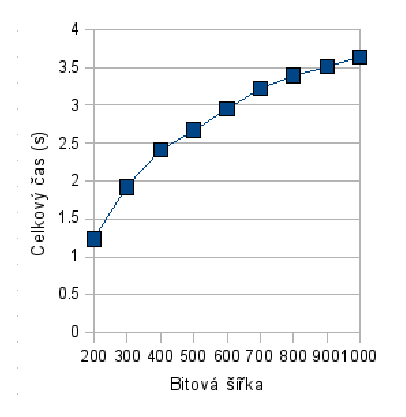
\includegraphics[width=5.0cm,keepaspectratio]{graph}
	\end{center}
\end{figure}

\noindent
Z~grafu jde názorně vidět, že nárust času vzhledem k~velikosti instance je
logaritmický, což odpovídá časové složitosti zjištěné při teoretické analýze algoritmu.

\section{Závěr}

Během vypracování projektu byla dodržena všechna specifika daná zadáním.
Projekt byl úspěšně otestován na školním serveru \texttt{merlin.fit.vutbr.cz}
pomocí vlastního testovacího scriptu.

\subsection*{Metriky}

\noindent
Počet zdrojových souborů: 1 \\
Počet řádků kódu: 298 (bez prázdných řádků, včetně komentářů)

\begin{thebibliography}{77}
\small
\bibitem{1} Hanáček P., Přednášky do předmětu PRL, \url{https://www.fit.vutbr.cz/study/courses/PDA/private/}, [citováno 21.4.2009]
\end{thebibliography}

\end{document}
